%------------- Commandes utiles ----------------

\section{Quelques commandes}

Voici quelques commandes utiles :

\subsection{Image}
%------ Pour insérer et citer une image centralisée -----

\begin{figure}[H] %le H sert à fixer l'image à cette endroit dans le texte
    \center
    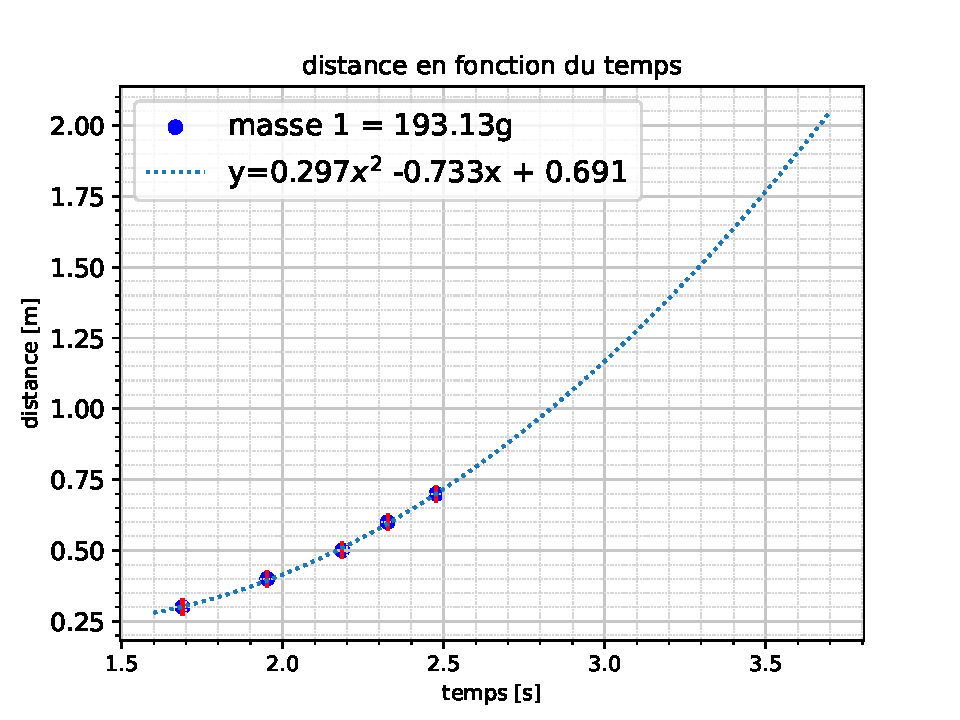
\includegraphics[width=16cm]{./logos/graph.pdf}
    \caption{Graphique}
    \label{Label de la figure}
\end{figure}

Ici, je cite l'image \ref{Label de la figure}.

\subsection{Équation}

%------- Pour insérer et citer une équation --------------

\begin{equation} \label{eq: exemple}
\rho + \Delta = 42
\end{equation}

L'équation \ref{eq: exemple} est cité ici. 

\subsection{Pythontex}
% ------- Pour écrire des variables ----------------------

Pour écrire des variables dans le texte, il suffit de mettre le symbole \$ entre le texte souhaité comme : constante $\rho$.

Pour utiliser pythontex :
\begin{pycode}
x = 3 #attention à l'indentation, il ne doit pas y avoir d'espaces avant la ligne
\end{pycode}
       
$x = \py{x}$

si x = ?? effectuer :
pythontex main.tex

Il est aussi possible d'écrire le code python dans autre fichier .tex
et l'inclure dans ce fichier.
\begin{pycode}
a = 23
b=4.23
c=2.2
d=3
e=0.3456
tableau_calc = '\\begin{tabular}{|c|c|c|c|c|}\n'
tableau_calc += '\\hline\n'
tableau_calc += '$a_1$ & $b_{test}$ & $c$ & d & $e$  \\\\ \\hline\n'
tableau_calc += f'{a} & {b} & {c} & {d} & {e} $m/s^2$\\\\ \\hline\n'
tableau_calc += '\\end{tabular}\n'
\end{pycode}

On peut aussi créer des tableaux latex en code python :

\begin{figure}[H]
    \centering
    \py{tableau_calc}
\end{figure}

Si il y a une erreur de compilation à cause du tableau,
comme celle-ci : Missing \$ inserted.

Supprimer le dossier pythontex-files-main et recompiler.

\subsection{Python}
Il peut être plus facile de créer des graphiques dans un fichier python séparé
et les sauvegarder comme images.

Un exemple de graphique (image \ref{Label de la figure}) a été crée avec python dans le dossier graph.